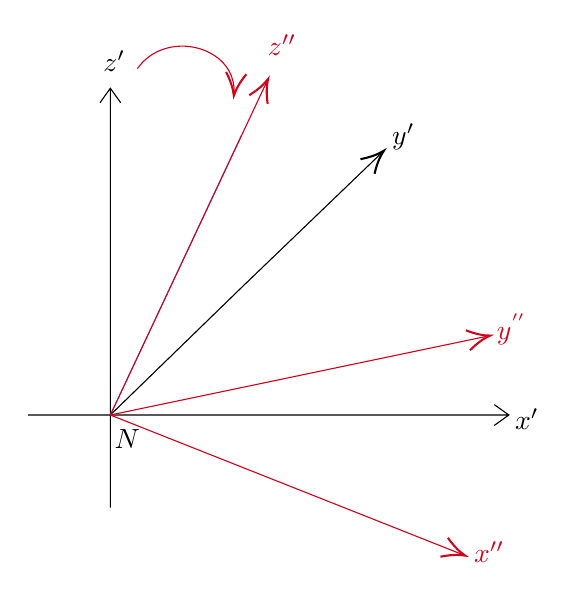
\begin{tikzpicture}[x=0.75pt,y=0.75pt,yscale=-1,xscale=1]
%uncomment if require: \path (0,373); %set diagram left start at 0, and has height of 373

%Shape: Axis 2D [id:dp09788258365708624] 
\draw  (138.44,245.33) -- (370,245.33)(178,87.89) -- (178,290) (363,240.33) -- (370,245.33) -- (363,250.33) (173,94.89) -- (178,87.89) -- (183,94.89)  ;
%Straight Lines [id:da3567635469042596] 
\draw [color={rgb, 255:red, 74; green, 144; blue, 226 }  ,draw opacity=1 ]   (178,245.33) -- (241.11,110.67) ;
%Straight Lines [id:da4078152355309548] 
\draw    (178,245.33) -- (241.11,184) ;
%Straight Lines [id:da7366378357929284] 
\draw    (241.11,184) -- (308.34,119.39) ;
\draw [shift={(309.78,118)}, rotate = 136.13] [color={rgb, 255:red, 0; green, 0; blue, 0 }  ][line width=0.75]    (10.93,-4.9) .. controls (6.95,-2.3) and (3.31,-0.67) .. (0,0) .. controls (3.31,0.67) and (6.95,2.3) .. (10.93,4.9)   ;
%Straight Lines [id:da4470005379087125] 
\draw [color={rgb, 255:red, 208; green, 2; blue, 27 }  ,draw opacity=1 ]   (178,245.33) -- (253.15,85.24) ;
\draw [shift={(254,83.43)}, rotate = 115.15] [color={rgb, 255:red, 208; green, 2; blue, 27 }  ,draw opacity=1 ][line width=0.75]    (10.93,-4.9) .. controls (6.95,-2.3) and (3.31,-0.67) .. (0,0) .. controls (3.31,0.67) and (6.95,2.3) .. (10.93,4.9)   ;
%Straight Lines [id:da7987238045742824] 
\draw [color={rgb, 255:red, 208; green, 2; blue, 27 }  ,draw opacity=1 ]   (178,245.33) -- (359.04,207.48) ;
\draw [shift={(361,207.07)}, rotate = 168.19] [color={rgb, 255:red, 208; green, 2; blue, 27 }  ,draw opacity=1 ][line width=0.75]    (10.93,-4.9) .. controls (6.95,-2.3) and (3.31,-0.67) .. (0,0) .. controls (3.31,0.67) and (6.95,2.3) .. (10.93,4.9)   ;
%Straight Lines [id:da33533616884876816] 
\draw [color={rgb, 255:red, 208; green, 2; blue, 27 }  ,draw opacity=1 ]   (178,245.33) -- (347.14,312.35) ;
\draw [shift={(349,313.08)}, rotate = 201.61] [color={rgb, 255:red, 208; green, 2; blue, 27 }  ,draw opacity=1 ][line width=0.75]    (10.93,-4.9) .. controls (6.95,-2.3) and (3.31,-0.67) .. (0,0) .. controls (3.31,0.67) and (6.95,2.3) .. (10.93,4.9)   ;
%Curve Lines [id:da5214771876679787] 
\draw [color={rgb, 255:red, 208; green, 2; blue, 27 }  ,draw opacity=1 ]   (191,78.48) .. controls (204.65,58.98) and (238.26,67.52) .. (237.62,89.74) ;
\draw [shift={(237.5,91.48)}, rotate = 276.07] [color={rgb, 255:red, 208; green, 2; blue, 27 }  ,draw opacity=1 ][line width=0.75]    (10.93,-4.9) .. controls (6.95,-2.3) and (3.31,-0.67) .. (0,0) .. controls (3.31,0.67) and (6.95,2.3) .. (10.93,4.9)   ;

% Text Node
\draw (178.8,251.13) node [anchor=north west][inner sep=0.75pt]    {$N$};
% Text Node
\draw (371.73,241.05) node [anchor=north west][inner sep=0.75pt]    {$x^{\prime }$};
% Text Node
\draw (312.53,103.85) node [anchor=north west][inner sep=0.75pt]    {$y^{\prime }$};
% Text Node
\draw (173.33,68.65) node [anchor=north west][inner sep=0.75pt]    {$z^{\prime }$};
% Text Node
\draw (252.6,61.05) node [anchor=north west][inner sep=0.75pt]  [color={rgb, 255:red, 208; green, 2; blue, 27 }  ,opacity=1 ]  {$z''$};
% Text Node
\draw (352,305.07) node [anchor=north west][inner sep=0.75pt]    {$\textcolor[rgb]{0.82,0.01,0.11}{x}\textcolor[rgb]{0.82,0.01,0.11}{''}$};
% Text Node
\draw (363,195.07) node [anchor=north west][inner sep=0.75pt]    {$\textcolor[rgb]{0.82,0.01,0.11}{y^{''}}$};


\end{tikzpicture}
